\usetikzlibrary{positioning,arrows}
\usetikzlibrary{decorations.pathmorphing}
\usetikzlibrary{decorations.markings}



\tikzset{
photon/.style={decorate, draw=black,
    decoration={coil,aspect=0}}
 }

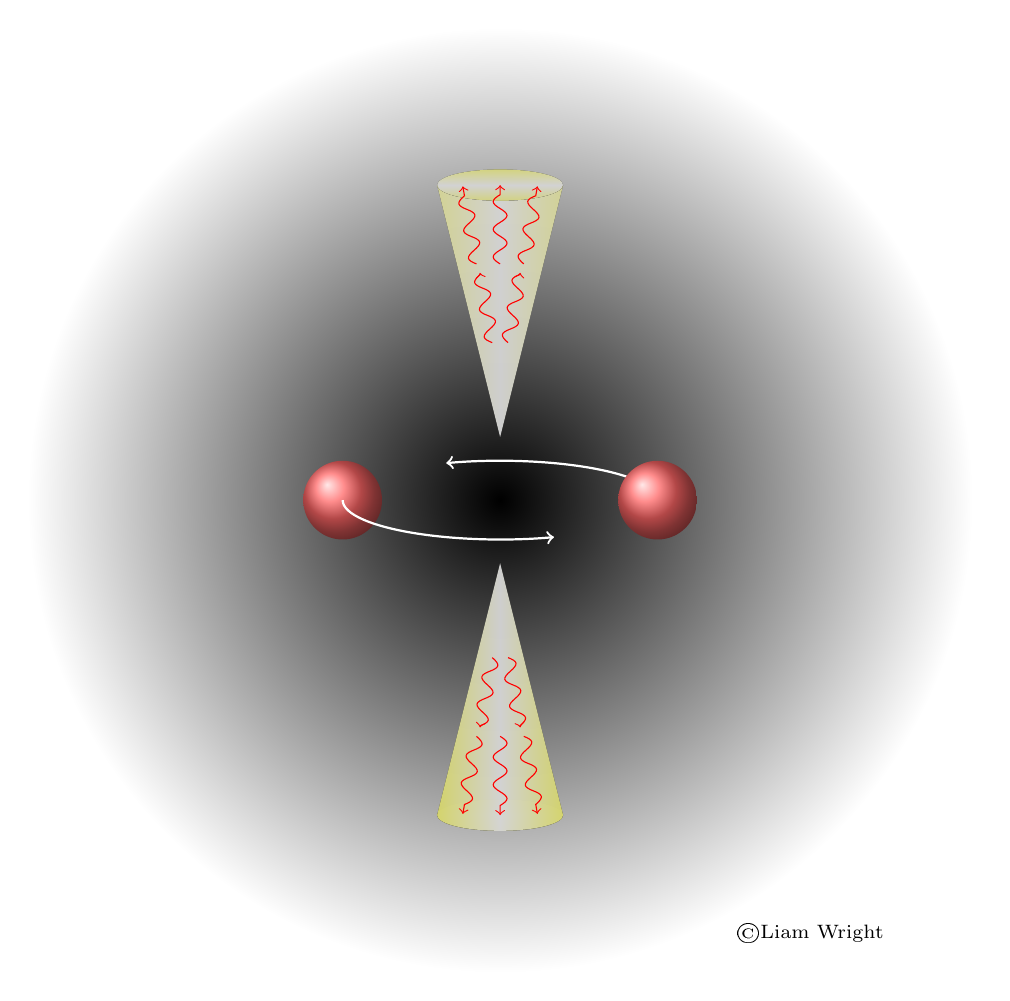
\begin{tikzpicture}


\shade[inner color=black, outer color=white] (0,0) circle (6);






\begin{scope}[scale=0.4]
\fill[top color=yellow!40!white,bottom color=yellow!40!white ,middle color=white,,opacity=.8] (0,-10) circle (2cm and 0.5cm);
\fill[left color=yellow!50!white,right color=yellow!50!white,middle color=white,opacity=.8] (2,-10) -- (0,-2) -- (-2,-10) arc (180:360:2cm and 0.5cm);

\fill[top color=yellow!40!white,bottom color=yellow!40!white ,middle color=white,,opacity=.8] (0,10) circle (2cm and 0.5cm);
\fill[left color=yellow!30!white,right color=yellow!30!white,middle color=white,opacity=.8] (2,10) -- (0,2) -- (-2,10) arc (180:360:2cm and 0.5cm);


\end{scope}


\begin{scope}[rotate=0]
\draw[photon, color=red, ->] (0,3) -- (0,4); 
\draw[photon, color=red, ->] (.1,2) --++(80:0.9); 
\draw[photon, color=red, ->] (-0.1,2) --++ (100:0.9); 
\draw[photon, color=red, ->] (0.3,3) --++ (80:1); 
\draw[photon, color=red, ->] (-0.3,3) --++ (100:1); 
\end{scope}

\begin{scope}[rotate=180]
\draw[photon, color=red, ->] (0,3) -- (0,4); 
\draw[photon, color=red, ->] (.1,2) --++(80:0.9); 
\draw[photon, color=red, ->] (-0.1,2) --++ (100:0.9); 
\draw[photon, color=red, ->] (0.3,3) --++ (80:1); 
\draw[photon, color=red, ->] (-0.3,3) --++ (100:1);
 \end{scope}


\draw[->, thick, color=white] (2,0) arc (0:110:2cm and 0.5cm);

\shade[ball color=white!40!red] (-2,0) circle (0.5);

\shade[ball color=white!40!red] (2,0) circle (0.5);
\draw[->, thick, color=white] (-2,0) arc (180:290:2cm and 0.5cm);

\node[text width=3cm, font = \scriptsize ] at (4.5,-5.5) {\textcopyright Liam Wright};

\end{tikzpicture} 	